\documentclass[12pt]{article}
%\renewcommand\normalsize{\fontsize{10pt}{12pt}\selectfont}
\usepackage{graphicx} % Required for inserting images
\usepackage[left=2cm,right=2cm,top=2cm,bottom=1.5cm]{geometry}

\title{HW 5, part 2}
%\author{Dennis Wilkinson}
\date{due Tuesday April 29}

\begin{document}

\setlength{\parindent}{0pt}
\setlength{\parskip}{3mm}

FS1 Spring 2025 Wilkinson
HW 5 Part 2

1. Go to https://animatedengines.com and look at (at least) the four stroke, two stroke, and steam locomotive engines. You can slow down the frame rate. The Newcomen atmospheric is actually the first ever engine; I think its efficiency is like 3\% or something.

2. It is easiest to calculate thermodynamic work $P\Delta V$ for \textit{isobaric} processes, where the pressure stays constant.

a. Why? (In the sense of, why is the calculation of $P\Delta V$ complicated for non-isobaric processes?)

One such isobaric process is boiling, in which 100 $^{\circ}$C water turns into 100 $^{\circ}$C steam. On Earth at sea level, for example, the water and steam are both at 1 atmosphere of pressure (or whatever the pressure is that day). 1 atm = 101300 Pa (pascals), where Pa = N/m$^2$ is the SI unit of pressure.

When water boils, it expands from a small volume in liquid form to a much larger volume as steam. This means it does thermodynamic work on its surroundings as it expands, which is one of the reasons we have to add heat to water to make it boil. In this problem we'll calculate the thermodynamic work of water turning into steam.

b. Find the mass of one mole of H$_2$O molecules in kg (if you remember from chemistry how to do this... otherwise read about it). Then calculate the volume of the liquid water in m$^3$; pure liquid water has density 958 kg/m$^3$ at 100 $^{\circ}$C and 1 atm. Density = mass/volume (divide, not multiply! Sorry). It will be very small, since one m$^3$ is large. 

c. Calculate the volume of 1 mole of 100 $^{\circ}$C steam at 1 atm of pressure using $PV=nRT$. 

d. Now calculate $P\Delta V$ for the water turning to steam. You'll need to use m$^3$ as the units for volume, and Pa for the pressure.

e. The \textit{latent heat of vaporization} is the amount of energy required to turn a substance from liquid to gas. For water at 1 atm it's 40800 J/mole. Compare this to your answer from (d). Your (d) should be a lot lower. Anyone want to guess why - where is the extra energy going when we boil water, besides to thermodynamic work? If not, read about it.

3. The following is a PV diagram showing an engine cycle. Process 3-1 is an adiabatic expansion, where (say) the gas is pushing a piston out.

\bigskip
\bigskip
\bigskip
\bigskip
\bigskip
\bigskip
\bigskip
\bigskip
\bigskip
\bigskip



a. Describe in words what is happening in processes 1-2 and 2-3. 

b. Say whether $W$, and $Q$, is positive, negative, or zero for each process. 

c. How does the PV diagram tell you the net work being done by the engine?

d. Let $T_1$, $T_2$, and $T_3$ be the temperatures at points 1, 2, and 3. Rank them from lowest to highest.


4. A Carnot cycle is a thermodynamic process which takes in heat at a fixed temperature $T_H$ and exhausts heat at a fixed temperature $T_C$. The Carnot cycle looks like this on a PV diagram:

\begin{figure}[h]
    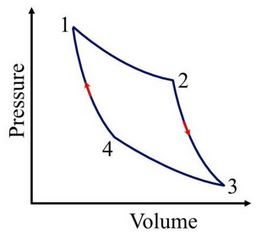
\includegraphics[width=0.4\linewidth]{Carnot PV.JPG}
\end{figure}

Processes 4-1 and 2-3 are adiabatic ($Q=0$) while 1-2 and 3-4 are isothermal processes ($T$ constant). 

a. Adiabatic expansion would be the part where the engine is pushing a piston out, quickly (so no heat flows, $Q=0$). Which leg of the cycle is this (1-2, 2-3, etc) in the diagram? The first law of thermodynamics states that $\Delta U = Q + W$ where $U$ is the internal energy, $Q$ is the heat flow, and $W$ is the thermodynamic work $P \Delta V$ done \textbf{on} the gas by external forces. Is $\Delta U$ positive, negative, or zero in the adiabatic expansion step? Does the gas get colder?

b. For each of the other three processes in the Carnot cycle, say whether each of $\Delta U$, $Q$ and $W$ is positive, negative, or zero. Use the convention that $W>0$ for work done on the gas (compression). Try to describe what is happening in each step.

c. In the Carnot process, $T_H$ is the temperature of the hot isothermal process, and $T_C$ of the cold. Is point 2 at $T_H$ or $T_C$? Calculate this temp if $P_2=150000$ Pa and $V_2=0.004$ m$^3$, and the number of moles of gas is $n=0.15$. 

d. The efficiency of an engine is the ratio of work out to heat in. For the Carnot process it's $\frac{T_H-T_C}{T_H}$. Explain why the efficiency is lower when $T_C$ and $T_H$ are closer to each other, in terms how we are getting work out of the gas.

e. Imagine a modern coal power plant with temp around 600 $^{\circ}$C in its boiler, where steam is heated; after pushing a turbine, the steam's temp falls to around 150 $^{\circ}$C. What's the Carnot efficiency for these temperatures (you must use Kelvin)? In fact, the best efficiency in coal plants is supposedly around 45\%, if you believe the manufacturers. Not too far off. (Then again, a coal plant process is not reversible, so it could theoretically be higher than the Carnot efficiency.)



 

\newpage

5*. A Stirling engine is a simple and elegant engine. There are various types, but the theoretical PV cycle for a simple Stirling engine is the following:

\begin{figure}[h]
    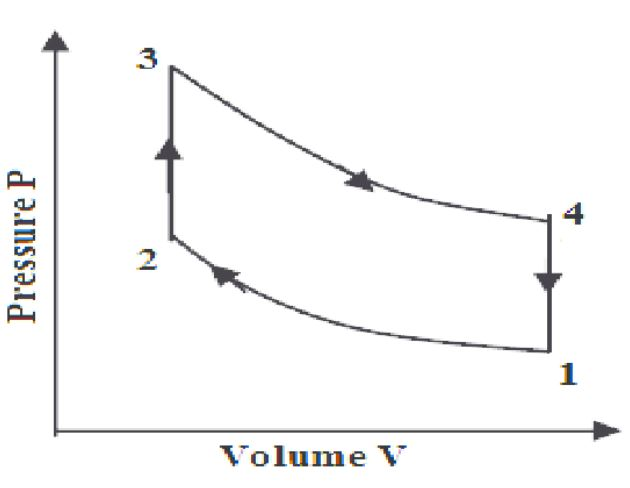
\includegraphics[width=0.5\linewidth]{Stirling PV.JPG}
\end{figure}

The cycle is similar to an Otto cycle, except that the expansion and compression are isothermal (constant $T$), not adiabatic. In this problem we calculate the efficiency $\eta = \frac{Q_{in}}{W}$.

The Stirling cycle has two reference temperatures, a high temp $T_H$ for the points along the 3-4 isotherm, and a low temp $T_C$ for the 1-2 isotherm. There are also two reference volumes, the small volume $V_2$ along 2-3 and a large volume $V_4$ along 4-1. 

a. Show that the net work  $\int P dV$ done in the Stirling cycle, per mole of gas, is $R \ln\frac{V_4}{V_2}(T_H-T_C)$. 

Heat is being input in two processes, 2-3 and 3-4. 

b. For the 2-3 process, we need a relation between the internal energy and the temperature. It's $\Delta U= nRC_V\Delta T$, where $C_V$ is called the molar specific heat at constant volume. With this, find $Q_{23}=RC_V(T_H-T_C)$ per mole.

c. Find the other input heat, $Q_{34}$, in terms of the temps and volumes, and finally,
\begin{equation}
\eta = \frac{T_H-T_C}{T_H+\frac{C_V(T_H-T_C)}{R \ln V_4/V_2}}
\end{equation}
for the cycle.

d. For ideal diatomic gases like air (mostly), $C_V=5R/2$. Use a reasonable ratio of volumes $V_4/V_2$ (this is called the \textit{compression ratio}) and calculate the Stirling efficiency if $T_H=400$ and $T_C=300$. Compare to Carnot. Under what conditions would the Stirling efficiency approach the Carnot efficiency?

The Stirling efficiency is actually greater than what we have calculated, because a good Stirling engine has a \textit{regenerator} which stores heat during the cycle. Stirling engines can have a (theoretical) efficiency equal to Carnot, but I have never done the calculation.
\end{document}